\part{Dataset Labelling}
%%%%%%%%%%%%%%%%%%%%%%%%%%%%%%%%%%%%%%%%%%%%%%%%%%%%%%%%%%%%%%%%%%%%%%%%%
% Dataset Labelling                                                     %
%%%%%%%%%%%%%%%%%%%%%%%%%%%%%%%%%%%%%%%%%%%%%%%%%%%%%%%%%%%%%%%%%%%%%%%%%
\section{Motivation and background}
This project is intimately linked with the neural networks project, but since a lot of time has been dedicated towards it, it merits a section for itself. This project is aimed at tackling the issue of lack of data, by providing a mechanism to get more data easily. The current bottleneck in aquiring more data is labelling the data, it's conceivably easy to set up a system to video hand washing, but to label it requires a bespoke system. This project is part of a broader initiative at Surewash to reevaluate the core computer vision system, and this project is part of the new testing framework. Surewash is collaborating with a group of researchers in Trinity, and the idea is to pool resources to develop reliable tools for marking up data for a computer system, as well as tools for evaluating the performance of the computer system.

Since this is a collaboration, the specification of this project is designed to meet the requirements of both Surewash, as well as the researchers at Trinity. The broad definition therefore of this project is a tool that could read in the data from an Intel Realsense camera, mark individual frames or segments of video as being part of $n \in \mathbb{N}$ classes, as well as marking an arbitrary amount of region of interests, hereby ROIs. There also had to be a way of comparing differant people's markup. There were no constraints on the implementation of the project, although it is desirable in my opinion to make a cross-platform solution. The end programme did have to work on Windows at the very minimum.

This project was assigned to both myself, as well as my fellow intern Gaurav. Since we're both somewhat familiar with Python and web development, we decided to use those tools to develop the solution. We agreed that I was more familiar with Python, and OS level scripting, so I mainly focused my efforts on server-side development, writing the programme for comparing marked up data, and any other miscellaneous scripts that handled file operations. Gaurav directed most of his attention towards writing the client-side code, such as the user interface.

Since this project is relatively unique, the specification and scope gradually increased as we developed the project. There were three stages to the development of the project. Initially, we developed a Flask application that labelled the an entire video in one sweep, marking ROI, and all possible classes at the same time (the user could mark ROI, then rewind the video, and mark up classes). The problem is that this approach only works for a small amount of classes. In Surewash, there are a total of twenty-four recocnised poses, and it is not reasonable to ask a marker to distinguish between all of these classes. These twenty four poses can together i.e. there are seven distinct poses, some of those poses are left or right-handed, some of those have variations depending on the orientation of a hand etc., so a solution needed to be found to mark the data in layers. In order to keep the complexity of the application to a minimum, I made the decision to develop a seperate wrapper Python application that would interface with the Flask application using an IPC pipeline. In short, the hierarchy of class labelling is laid out in a heirarchal folder structure (using the file system provided by the host OS), at the core of the wrapper application (hereby the backend) was a recursive function that moves through this file strucure and uses the layout to interface with the Flask application. This layout allowed myself and Gaurav to work indepedently, I worked on the backend application, while Gaurav continued to work on the Flask application.

%%%%%%%%%%%%%%%%%%%%%%%%%%%%%%%%%%%%%%%%%%%%%%%%%%%%%%%%%%%%%%%%%%%%%%%%%
% Overview                                                              %
%%%%%%%%%%%%%%%%%%%%%%%%%%%%%%%%%%%%%%%%%%%%%%%%%%%%%%%%%%%%%%%%%%%%%%%%%
\section{Overview Of Programme}
The process of labelling the data is divided into two distinct stages, first process and label the data, then compare the markup of the labelled data between differant people.
    \subsection{Preprocessing and labelling}
    The data is captured on an Intel Realsense camera, which saves the data in ROS-bag format which is an uncompressed video \cite{intelrosbag}. This needs to be converted into an ordinary video format (such as MPEG-4 \cite{wiegand2003overview}). There is a tool within the library of the Realsense camera which converts to still PNG images \cite{boutell1997rfc}, another tool called FFMPEG \cite{ffmpeg} is used to convert to MPEG-4. 
    
    This programme is conceptually divided into two parts, the data is labelled in a GUI web app, and there is another backend programme that interfaces with the GUI web app. In the GUI web app, the user can play the video (or press a button to advance one frame at a time), and a series of buttons can be pressed while looking at the video to mark it as belonging to a particular class, see Figure \ref{fig:markupscreenshot}. The user can also mark ROI by dragging a bounding box on the video. Pressing {\slshape Next} terminates the web server and the server outputs the markup as a character sequence representation of a Python list (see below for details) to the standard output. The particular binary formatting of that string depends on what the host operating system uses (I found that my computer uses UTF-8 \cite{yergeau1996utf}). When the Flask app is starting, it has a flag that can be set such that it also accepts data pre-marked in the standard input (using a similar character sequence).

    The Flask app dynamically generates the class buttons by looking in a particular folder for images. For example, it it looks in its photo directory and finds three images, it will show three buttons on the web page, the class type is determined by the file name of the image, so in this example, they should be called {\slshape 1.png}, {\slshape 2.png}, and {\slshape 3.png}. The video path is specified in an argument to the programme.

    The core role of the wrapper application is to interface with the Flask application and seamlessly faciliatate the markup of the classes, as well as subclasses. After the top layer of class markup is complete, inspects the markup, calculates the sections of video that need to be marked with sub-classes, and then appropriately crops the original video before sending it to the flask app. In the context of Surewash, after the user has marked the seven top-level poses, the next task will be to mark the sub classes of pose two, so it will crop the video to only display the sections of video containing pose two (which can be an arbitrary amount of arbitrary sections of the video), and then send this video back to the flask app, as well as the appropriate class buttons. The loading, and reloading of the browser is facilitated using Selenium.

    % \begin{tikzpicture}[node distance=11cm]
    %     \node (wrapper) [process] {Wrapper};
    %     \node (flask) [process, right of=wrapper] {Flask};
    %     \draw [arrow] (wrapper.170) -- node[anchor=south] {Classes (multiple .png files),\\
    %      Video (one .mp4 file),\\ 
    %      Current markup (std input)} (flask.10);
    %     \draw [arrow] (flask.350) -- node[anchor=north] {Markup} (wrapper.190);
    % \end{tikzpicture}        

    \begin{figure}[h]
        \centering
        \fbox{ 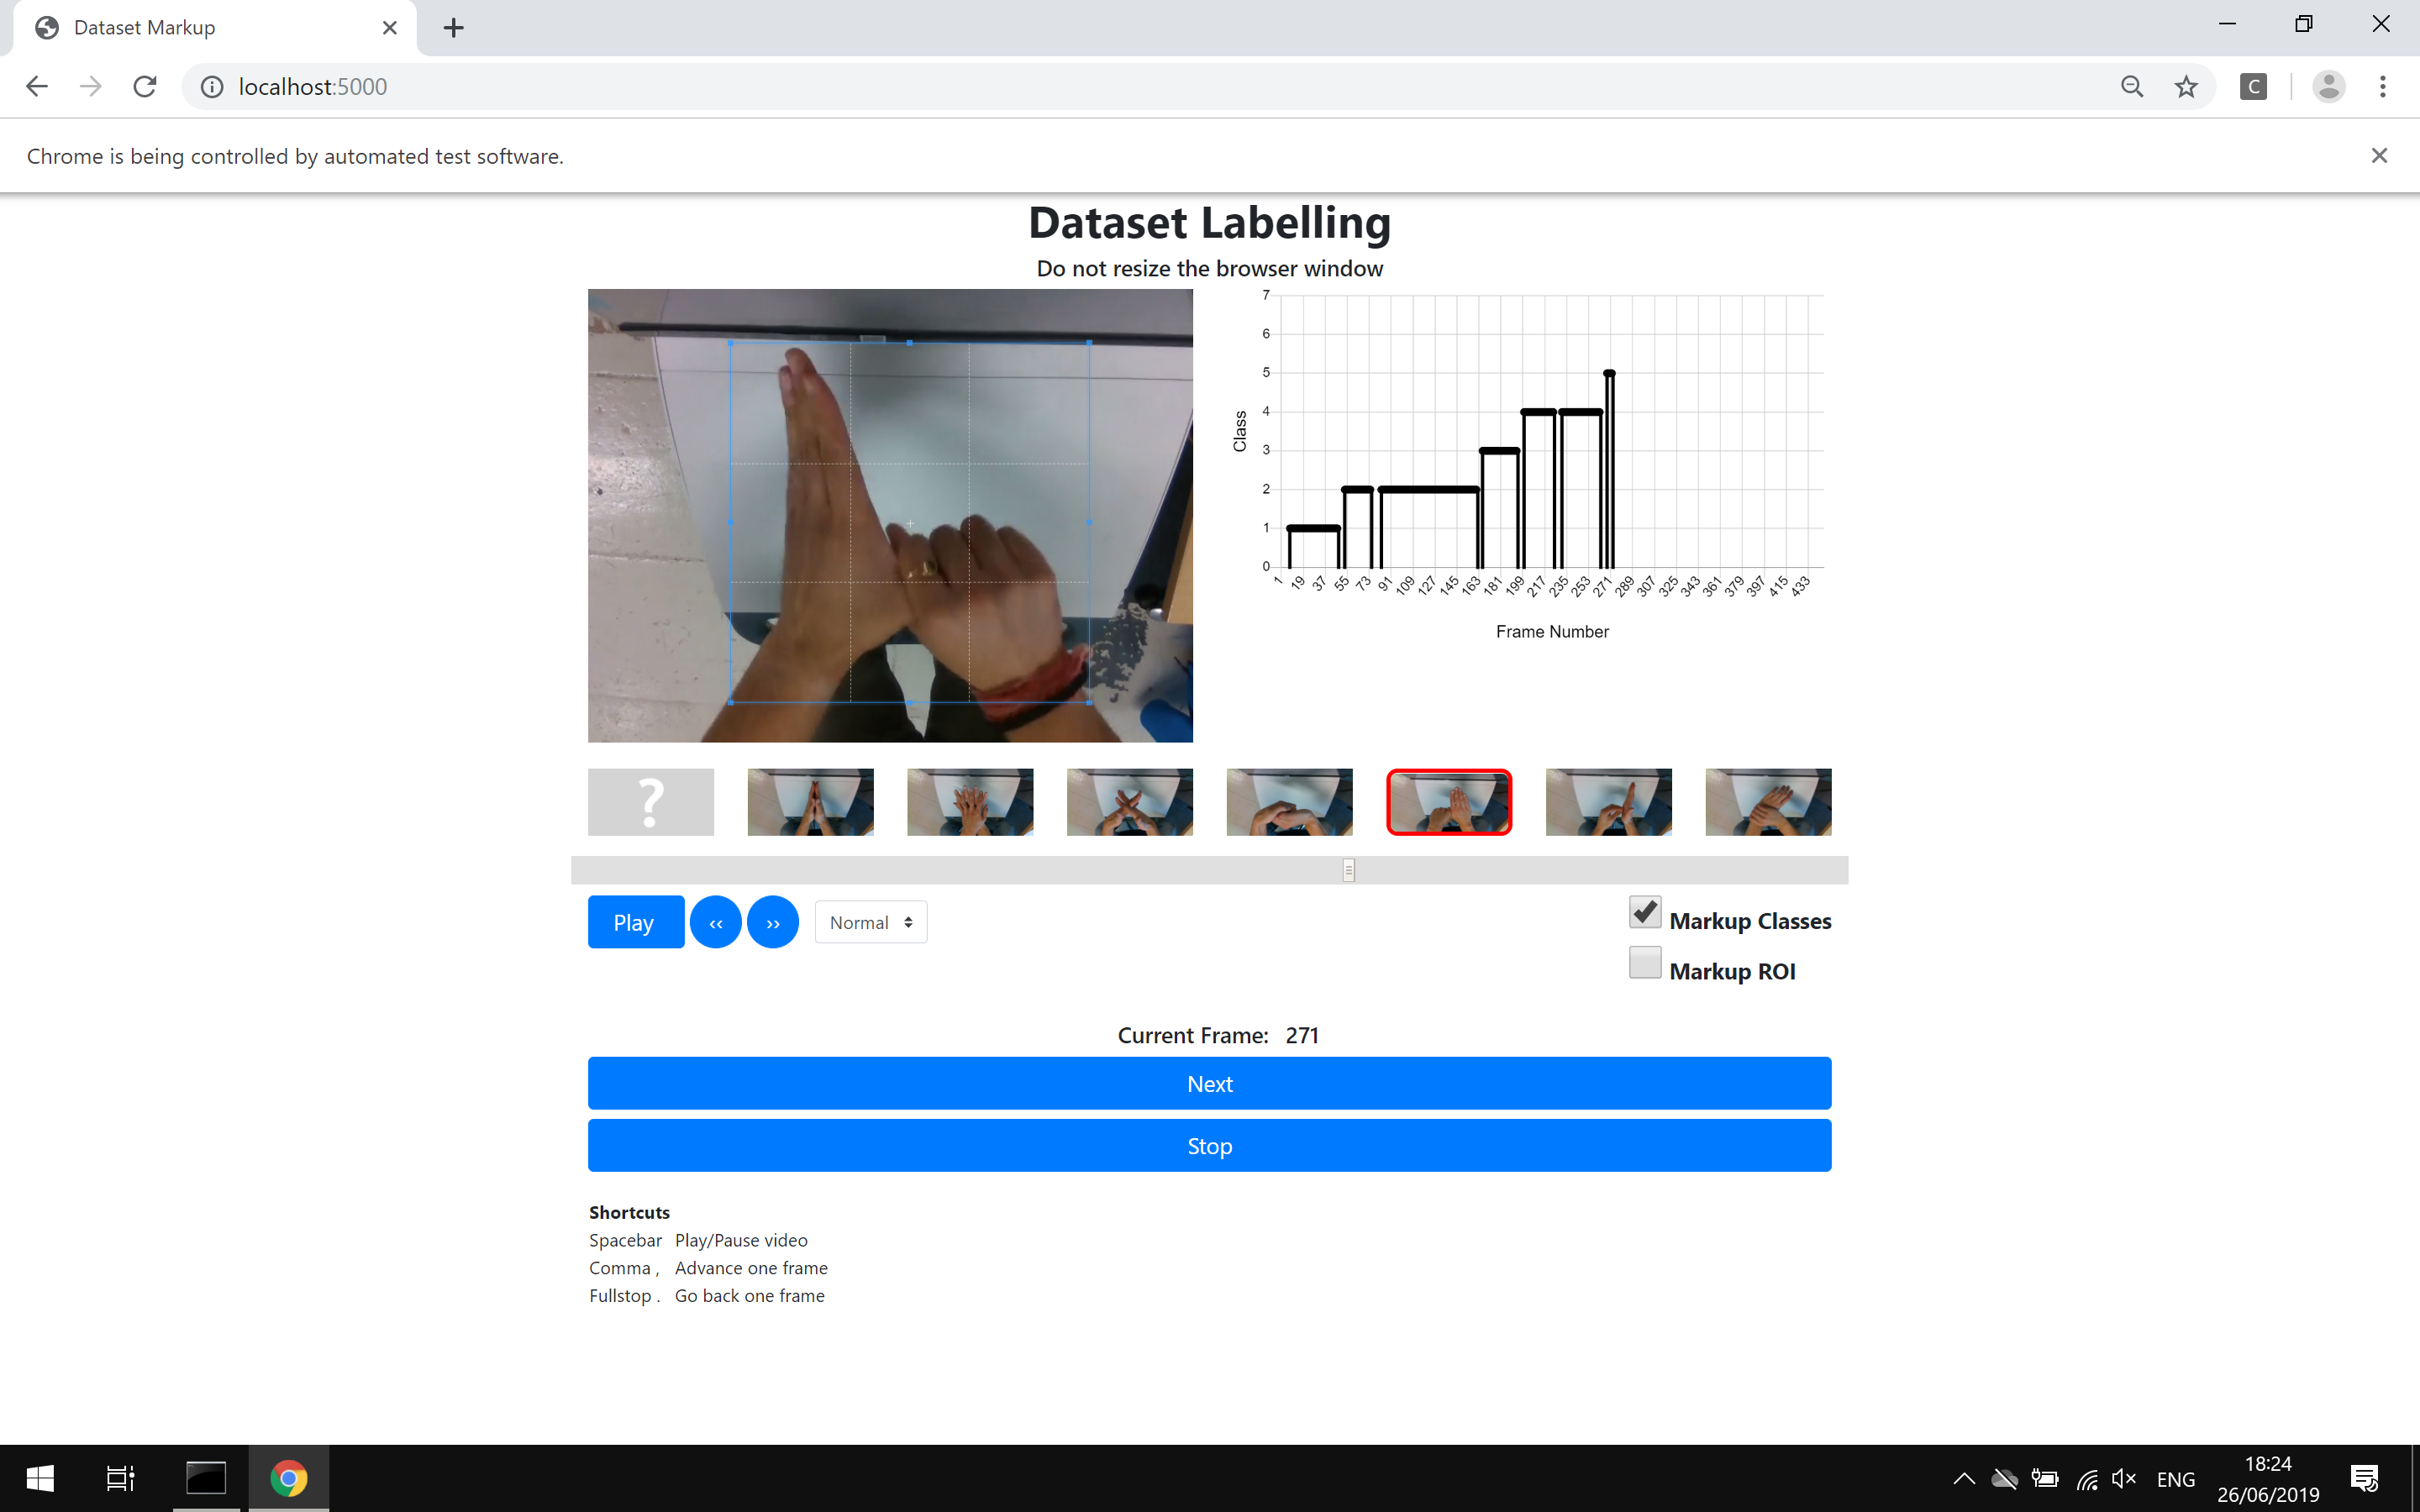
\includegraphics[width=450px]{../img/markup_screenshot.png} }
        \caption{Screenshot of the labelling web app, all images are \copyright \space Glanta DAC (note that the browser was zoomed out to 67\% to fit the screenshot)}
        \label{fig:markupscreenshot}
    \end{figure}

    \subsection{Comparison} 
    It is likely that at least some errors will be made in the labelling step, therefore this step will assume that at least two differant people performed labelling on the same video, or at least the same person did the labelling twice. A programme was written that will compare two differant markup files, and it will report where there was disagreements between two markup files so that they can be looked at again.

%%%%%%%%%%%%%%%%%%%%%%%%%%%%%%%%%%%%%%%%%%%%%%%%%%%%%%%%%%%%%%%%%%%%%%%%%
% Technical details                                                     %
%%%%%%%%%%%%%%%%%%%%%%%%%%%%%%%%%%%%%%%%%%%%%%%%%%%%%%%%%%%%%%%%%%%%%%%%%
\section{Technical Details}
    %%%%%%%%%%%%%%%%%%%%%%%%%%%%%%%%
    % Backend                      %
    %%%%%%%%%%%%%%%%%%%%%%%%%%%%%%%%
    \subsection{Labelling - Backend}
    The backend is a Python script, it controls the frontend by launching it as a seperate process using the Python {\slshape Subprocess} module. During the lifecycle of the backend, for each video, it starts, and stops the frontend process multiple times mark the differant classes. The heirarchy of class labelling that I choose in consultation with my superviser is as follows (each box represents a folder).\\

    \begin{tikzpicture}[node distance=2cm]
        \node (p1) [posebox]			    {1};

        \node (p2) [posebox, right of=p1]	{2};
            \node (p21) [posebox, below of=p2, xshift=-1.6cm]	{2, 1};
                \node (p211) [posebox, below of=p21, xshift=-0.6cm]	{2, 1, 1};
                \node (p212) [posebox, below of=p21, xshift=0.8cm]	{2, 1, 2};
            \node (p22) [posebox, below of=p2, xshift=-0.2cm]	{2, 2};
                \node (p221) [posebox, below of=p22, xshift=0.8cm]	{2, 2, 1};
                \node (p222) [posebox, below of=p22, xshift=2.2cm]	{2, 2, 2};

        \node (p3) [posebox, right of=p2]	{3};

        \node (p4) [posebox, right of=p3]	{4};
            \node (p41) [posebox, below of=p4, xshift=-2.0cm]	{4, 1};
            \node (p42) [posebox, below of=p4, xshift=-0.6cm]	{4, 2};

        \node (p5) [posebox, right of=p4]	{5};
            \node (p51) [posebox, below of=p5, xshift=-1.2cm]	{5, 1};
                \node (p511) [posebox, below of=p51, xshift=-1.4cm]	{5, 1, 1};
                    \node (p5111) [posebox, below of=p511, xshift=-0.7cm]	{5, 1, 1, 1};
                    \node (p5112) [posebox, below of=p511, xshift=0.7cm]	{5, 1, 1, 2};
                \node (p512) [posebox, below of=p51, xshift=0.0cm]	{5, 1, 2};
            \node (p52) [posebox, below of=p5, xshift=0.2cm]	{5, 2};
                \node (p521) [posebox, below of=p52, xshift=0.0cm]	{5, 2, 1};
                    \node (p5211) [posebox, below of=p521, xshift=-0.7cm]	{5, 2, 1, 1};
                    \node (p5212) [posebox, below of=p521, xshift=0.7cm]	{5, 2, 1, 2};
                \node (p522) [posebox, below of=p52, xshift=1.4cm]	{5, 2, 2};

        \node (p6) [posebox, right of=p5]	{6};
            \node (p61) [posebox, below of=p6, xshift=-0.4cm]	{6, 1};
            \node (p62) [posebox, below of=p6, xshift=1.0cm]	{6, 2};

        \node (p7) [posebox, right of=p6]	{7};
            \node (p71) [posebox, below of=p7, xshift=0.4cm]	{7, 1};
                \node (p711) [posebox, below of=p71, xshift=-1.4cm]	{7, 1, 1};
                \node (p712) [posebox, below of=p71, xshift=0cm]	{7, 1, 2};
            \node (p72) [posebox, below of=p7, xshift=1.8cm]	{7, 2};
                \node (p721) [posebox, below of=p72, xshift=0cm]	{7, 2, 1};
                \node (p722) [posebox, below of=p72, xshift=1.4cm]	{7, 2, 2};

        \draw [arrow] (p2) -- (p21);
            \draw [arrow] (p21) -- (p211);
            \draw [arrow] (p21) -- (p212);
        \draw [arrow] (p2) -- (p22);
            \draw [arrow] (p22) -- (p221);
            \draw [arrow] (p22) -- (p222);

        \draw [arrow] (p4) -- (p41);
        \draw [arrow] (p4) -- (p42);

        \draw [arrow] (p5) -- (p51);
            \draw [arrow] (p51) -- (p511);
                \draw [arrow] (p511) -- (p5111);
                \draw [arrow] (p511) -- (p5112);
            \draw [arrow] (p51) -- (p512);
        \draw [arrow] (p5) -- (p52);
            \draw [arrow] (p52) -- (p521);
                \draw [arrow] (p521) -- (p5211);
                \draw [arrow] (p521) -- (p5212);
            \draw [arrow] (p52) -- (p522);

        \draw [arrow] (p6) -- (p61);
        \draw [arrow] (p6) -- (p62);

        \draw [arrow] (p7) -- (p71);
            \draw [arrow] (p71) -- (p711);
            \draw [arrow] (p71) -- (p712);
        \draw [arrow] (p7) -- (p72);
            \draw [arrow] (p72) -- (p721);
            \draw [arrow] (p72) -- (p722);
        
    \end{tikzpicture}

    The core of the backend application is a recursive function that parses through this heirarchal structure. For the above example, when the user starts the backend application, the recursive function starts at the top of this structure, so when the web browser opens, they will see seven buttons, to label the classes from 1-7 (like in \ref{fig:markupscreenshot}). The video that was served to the frontend will be cropped into five sections, since classes 2, 4, 5, 6, and 7 contain sub classes tp label (in this context, these subclasses denote whether the pose is left, or right handed). From the root call of the recursive function, it will thus make five calls to itself to label the subsections of classes 2, 4, 5, 6, and 7. When the next layer of class 2 has been labelled, the second layer of the recursive function will call itself twice to label those two subsections. When this process is finished, the end result will a video that is labelled with up to twenty differant classes, as well as sections that are marked ambiguous (a transition between a class is an example of a section of video that might be marked as ambiguous).

    \paragraph{Video processing}
    The videos that this programme marks up come in the ROS-bag format, which as mentioned above is a special format of video used by the Realsense camera which is not compatible with a web browser, thus a central task of the backend is to convert this video to a more common standard, and MPEG-4 H.264 is what the backend converts to. A tool is included in the Realsense SDK that converts a .bag file to a series of PNG images, so before the recursive function is called, this ROS-bag converter is called to do this, and then a folder containing the sequence of PNG files is kept for the duration of the video's markup. When calling the recursive function, one of the arguments contains the sections of video that is to be marked up, (e.g. that could be [[0, 150]] to label frames 0-150, or [[43, 87], [92, 104]] to label frames 43-87 and 92-104). The first thing that the recursive function does therefore is to make a series of videos based on the segments supplied to it, and then concatenate these videos, which is then sent to the frontend. The video is sent to the frontend by moving it to the static/videos/video.mp4 folder, and specifying that path in the arguments for launching the frontend.

    \paragraph{Segmenting markup}
    The backend crops the video for child calls of the recursive function based on how the user marked up the video, so it needs a way to process the markup, and find the segments of video that will be used for sub-labelling. No assumptions can be made on the composition of the video e.g. whether the sequence of classes will always be the same, whether all, or only some classes are present, whether the region of video contains a particular class is continuous. Figure \ref{fig:labelsample} can be used an example, there are some sections that have been marked as ambiguous (and thus do not need any further labelling), not all classes appear in this video, and some sections are not continuous.

    \begin{figure}[h]
        \centering
        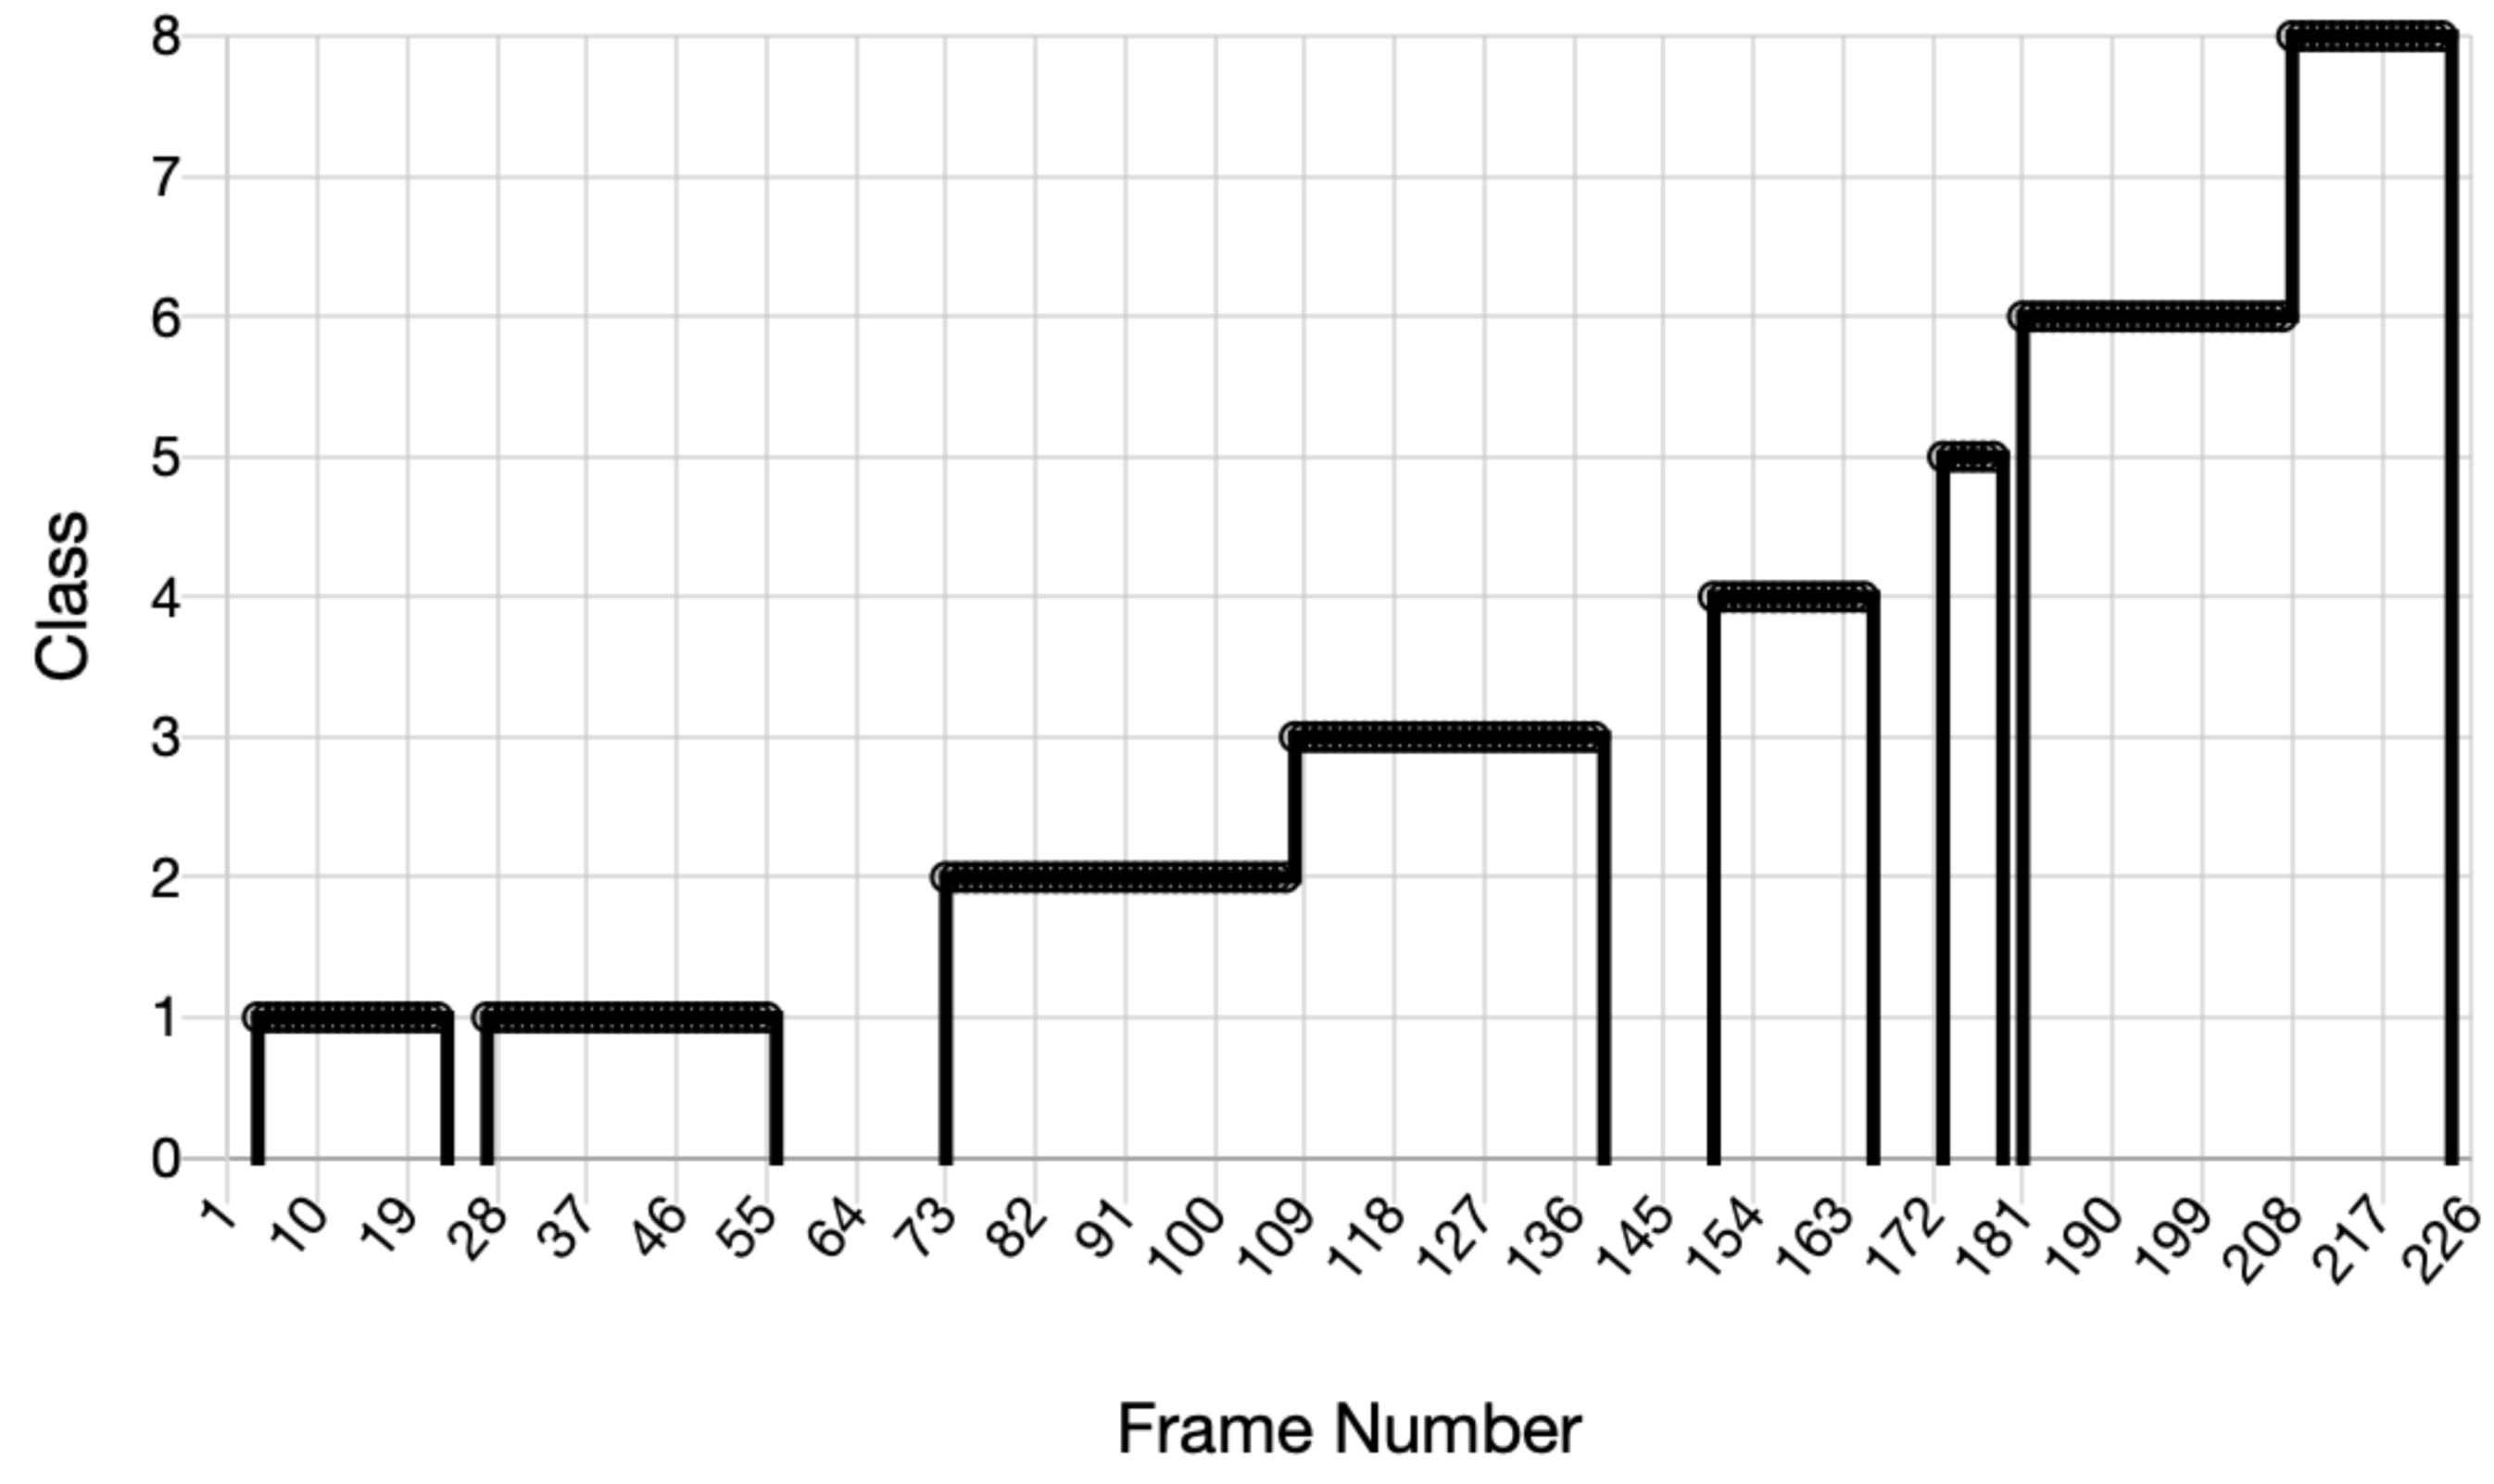
\includegraphics[width=450px]{../img/sample_label.png}
        \caption{A sample markup for a video}
        \label{fig:labelsample}
    \end{figure}

    When the backend receives the results from the frontend, it passes this an list to a function to segment the results, where each index corresponds to a frame number, and its value is the class that that frame is marked as. The results are segmented by first binning the frame numbers into a python dictionary, where the key is the class, and the values for each key are the frame numbers, these values are sorted into ascending order. Each list entry in the dictionary is then converted to a list containing lists that show the start, and end frame for that class.
    \begin{lstlisting}[style=PythonStyle]
    # The ROI has been ommitted from results for convenience
    # Assume that there are only two classes to mark
    # Each index in results corresponds to a frame number
    results = [-1, -1, 1, 1, 1, 1, -1, 2, 2, 2, -1, 2, 2, 2, 2]
    binned_results = {
    -1: [0, 1, 6, 10],
    1:  [2, 3, 4, 5],
    2:  [7, 8, 9, 11, 12, 13, 14]
    }
    segmented_results = {
    -1: [[0, 1], [6, 6], [10, 10]],
    1:  [[2, 5]],
    2:  [[7, 9], [11, 14]]
    }\end{lstlisting}
    The ambiguous sections (-1) would be discarded, and two sub-videos would be made, one containing frames two to five, and one containing the concatenated frames of seven to nine, and eleven to fourteen.

    \paragraph{Saving progress mid-labelling}
    A feature request of the backend is that the user could stop in the middle of labelling a video, return at a later time, and come back to the same state. In Python, when a programme is signalled to stop mid-execution, a {\slshape KeyboardInterrupt} exception is thrown, and this exception is caught to save the state. In the normal execution of the recursive function, when it finishes, it returns an empty list, but if it ends with a {\slshape KeyboardInterrupt} being thrown, a list with the frame intervals is included in the return value, then the parent recursive calls appends the segmented results dictionary described above, as well as the list of frame intevals that it is labelling (the top level call will have a frame interbal of [[0, maximum\_frame]]). Extending the above example, if the subclasses of class 2 were being labelled and the user stopped the programme, the return value of the top level recursive function would be as follows.

    \begin{lstlisting}[style=PythonStyle]
    return_value = [[[7, 9], [11, 14]], { -1: [[0, 1], [6, 6], [10, 10]], 1:  [[2, 5]], 2:  [[7, 9], [11, 14]]}, [[0, 14]]]
    # summary: return_value = [frame_interval, segmented_results, frame_interval]
    # This is where there was one level of recursion, if there was two levels of recursion, it would look like this
    # summary: return_value = [frame_interval, segmented_results, frame_interval, segmented_results, frame_interval]
    # In general, the amount of levels of recursion is length((return_value - 1) / 2)\end{lstlisting}

    This return value, along with the results, and list of videos yet to be labelled are stored in file using Python's Pickle module (a built-in way of storing Python objects in File objects). When the user starts the programme again, if this Pickle file exists, it will reload the results, and call the recursive function again, and treat the return\_value variable as a stack. From the above example, it will know that the sub class of class 2 is nect to be labelled, because it can match [[7, 9], [11, 14]] with the key value 2 in the dictionary, and that class 1 has already been labelled because it calls itself in numerical order.

    \paragraph{Miscellaneous}
    For Surewash, my supervisor asked me to record videos at 30 frames/second, one problem with this is that a hand hygiene session usually takes 25-30 seconds or more, which corresponds to 750-900 frames. It was suggested that a preprocessing step could be taken to only label frames that are sufficiently differant from each other, but given the time constraints of the project, I determined that this would not be a feasible feature to implement, so a compromise is to only label every second frame. This option can be set by setting a boolean called {\slshape half\_frames} to True.

    A request of the researchers at Trinity was that more than one ROI region could be marked up, so an Integer value can be set to determine how many ROI regions are to be marked, this value is then passed to the frontend which formats the webpage appropriately.

    \paragraph{Final results}
    The actual output of the backend, the markup for each video is saved in JSON format \cite{bray2017rfc}. There is one file per ROS-bag file, each JSON file contains one JS object. The object contains key-value pairs for the video name, whether only every second frame was marked, the number of ROI, the date, the user who marked the video (determined from the Python {\slshape os.getlogin()} function which returns the name of the User account on the computer), as well as the data. The data is itself a JS object with key-value pairs for each frame. Each from is a JS object containing each ROI, as well as the class. Note that the below example ommitts frames 4-164 for the sake of brevity, the JSON file also does not contain any newline character sequences.

    \begin{lstlisting}[style=JSStyle]
{
    "VIDEO_NAME": "20190626_121748.bag", 
    "HALFFRAMES": false, 
    "NUM_ROI": 1, 
    "DATE": {"YEAR": 2019, "MONTH": 6, "DAY": 27, "HOUR": 10, "MINUTE": 1, "SECOND": 25}, 
    "USER": "Daniel", 
    "DATA": {
        "0": {"ROI": {"0": [0.23055555555555557, 0.3802469135802469, 0.7601851851851852, 0.9975308641975309]}, "CLASS": [2, 1, 1]},
        "1": {"ROI": {"0": [0.23055555555555557, 0.3802469135802469, 0.7601851851851852, 0.9975308641975309]}, "CLASS": [3]}, 
        "2": {"ROI": {"0": [0.23055555555555557, 0.3802469135802469, 0.7601851851851852, 0.9975308641975309]}, "CLASS": [4, 1]}, 
        "3": {"ROI": {"0": [0.23055555555555557, 0.3802469135802469, 0.7601851851851852, 0.9975308641975309]}, "CLASS": [4, 1]},
        ...
        "165": {"ROI": {"0": [0.23055555555555557, 0.3802469135802469, 0.7601851851851852, 0.9975308641975309]}, "CLASS": [3]},
}\end{lstlisting}

    %%%%%%%%%%%%%%%%%%%%%%%%%%%%%%%%
    % Frontend                     %
    %%%%%%%%%%%%%%%%%%%%%%%%%%%%%%%%
    \subsection{Labelling - Frontend}
    Since the front is a web app, the code is divided into two parts, the server code, and the client code. The layout of the output is as follows:

    \[
    \begin{bmatrix}
    (x_{10} & y_{10} & x_{20} & y_{20})_n & c_{0} \\
    (x_{11} & y_{11} & x_{21} & y_{21})_n & c_{1} \\
    (x_{12} & y_{12} & x_{22} & y_{22})_n & c_{2} \\
    (x_{13} & y_{13} & x_{23} & y_{23})_n & c_{3} \\
     \vdots & \vdots & \vdots & \vdots    & \vdots\\
    (x_{1n} & y_{1n} & x_{2n} & y_{2n})_n & c_{n} 
    \end{bmatrix}
    \]
    \begin{gather*}
    x, y \in \mathbb{R} [0, 1]\\
    c, n \in \mathbb{Z}
    \end{gather*}

    The $x$ and $y$ values represent coordinates describing an ROI box (top left, and bottom right), $n$ denotes how many ROI regions there are  to mark up (e.g. if there were two ROI regions to markup, there would be nine columns in the matrix, and thirteen columns if there were three columns to markup etc.), and the $c$ value represents the class (the classes must be encoded in integer form). Each row represents one frame. By default, all values are set to -1 to denote that they have either not been labelled, or are 'ambiguous'. The coordinates represent the ROI in a proportional system, so if the image is 350 pixels wide, and a $y$ coordinate was $0.22$, then that would refer to the 77th pixel. The coordinates are represented proportionally because the original video is scaled from the original BAG file, and since the ROI box does not have to be precisely correct, this system is acceptable in my opinion. In the markup file, the $x$ and $y$ values are represented by floating point values, and the class values are signed integers.

        \subsubsection{Server Code}
        This is primarily a Flask app \cite{flaskpocoo}. Flask is a Python web framework, similar in concept to Django but without the model layer, and web security features, which are not necesasary for this application. It is thus easier to write an application in Flask as opposed to Django. Flask applications are divided into two main areas, the view, and the template. The view is a series of functions that define HTTP POST and HTTP GET requests \cite{fielding1999hypertext}. When a HTTP request is made, if the response contains a body, the relevant template (which can contain a file with special escape sequences for adding variables defined in the view, including conditional formatting) is returned, with all of the escape sequences evaluated. In this context of this application, all of the template files are HTML files. The HTML page that the server serves to the client contains the path to the video to be marked (which is specified when starting the flask app from the backend application), it also formats the class buttons, based on what it sees in the {\slshape /static/classes} folder. Before the backend application starts the flask app, it copies the current classes to the classes folder.
        
        The server acts 'dumb', its main task apart from serving the client application initially to the web browser is to take the marked up data and save it, it does not do any processing with the data itself. The view exposes a HTTP GET, and HTTP POST method for downloading and uploading the markup data, as a fail-safe, the client also pushes the current markup every three seconds via a seperate HTTP POST request. As described above, when the user presses the {\slshape Next} button, it outputs the data to the standard output in a character sequence, which is followed by a ? delimiter, which is used instead of a newline character due to difficulties with it being formatted as a literal \\n, and not the os newline charater, using ? was a simple workaround. If the user presses the {\slshape Stop} button instead, the server is also stopped, but at the end of the character sequence, `STOP?' is appended, which signals to the backend application to stop and save the progress to resume at a later time.

        \subsubsection{Client Code}
        All of the logic for marking up the data happens in the client code, and since this is a web application, all of this code is written in JavaScript. The results are stored in an array of arrays. Each entry in the parent array corresponds to a frame, and each array in that corresponds to the coordinates, and class for that frame. Every time the video is played, paused, its frame put forward, or backward, it triggers a method to push the array back to the server using a Jquery AJAX method.

            \paragraph{Classes}
            The class is marked simply by pressing a button for what the class is for the currently displayed frame, it finds the buttons by looking in an appropriate directory within the app folder. The currently displayed frame is obtained with the following function:
                \begin{lstlisting}[style=JSStyle]
function return_current_frame() {
    var curr_frame = Math.floor(theVideo.currentTime*frameRate);
    if(curr_frame >= frame_count) {
        curr_frame = frame_count - 1;
    }
    return curr_frame;
}\end{lstlisting} 
            Since HTML5 video does not expose a way to get the frame number directly, it has to be obtained by multiplying the current time by the frame rate. Since there also is no way of determening the frame rate directly, a server-side HTTP GET method is used which uses ffprobe to determine the frame rate and push that to the client side using a Jquery AJAX method.

            \paragraph{ROI}
            Finding a way to mark ROI from a web browser is more difficult, since there weren't any out of the box solutions that existed as far as I could see. The solution involved using a Javascript library called Cropper.js \cite{cropperjs}. This library is designed to load an image in for marking an area to crop. It was adapted to this solution by overlaying it on the video using some CSS, and every time the video frame changed, the current cropped coordinates were obtained and saved to the results matrix. The method of overlaying led to issues with the coordinates that it outputted did not correspond to the video resolution due to the nature of this solution. The $x$ coordinates ranged from 0, to the width of the HTML5 canvas element, which means that this can be converted to proportional coordinates (mentioned above) easily. The $y$ coordinates on the other hand presented more issues, since they ranged from approximately $[-9.44, 159.31]$ using a 16:9 aspect, and I could not source a reasonable explanation as to why this was the case. This quirk was consistent across browers and operating systems. The initial solution to convert the $y$ coordinates to proportional coordinates was to them to a line with $y=mx+c$ using the coordinates $(-9.44,0)$ and $(159.31,1)$. To prevent edge cases straying above 1, or below zero, the output values were clamped between these two values. The final code to do the conversion looks like the following. This solution did not work for differant aspect ratios however. After trial, and error, I found that the height of the video was directly proportional to the aspect ratio, so in the below example, a 4:3 aspect ratio for the video meant that it would have a total height of 225, and if the aspect ratio was changed to 16:9, it could be calculated by obtaining by using that aspect ratio.

            \begin{lstlisting}[style=JSStyle]
function get_proportional_coordinates(cropper_instance, x1_func, y1_func, x2_func, y2_func) {
    var curr_width = cropper_instance.getCanvasData().naturalWidth;
    var natural_height = cropper_instance.getImageData().naturalHeight;
    var gross_height = ( (225 / (405 / 540) ) * ( cropper_instance.getContainerData().height / cropper_instance.getContainerData().width ) );
    var overspill = (gross_height - natural_height) / 2;

    var y1_proportional = (y1_func + overspill) / gross_height;
    var y2_proportional = (y2_func + overspill) / gross_height;
    var x1_proportional = x1_func / curr_width;
    var x2_proportional = x2_func / curr_width;

    if      (y1_proportional > 1)   y1_proportional = 1;
    else if (y1_proportional < 0)   y1_proportional = 0;

    if      (y2_proportional > 1)   y2_proportional = 1;
    else if (y2_proportional < 0)   y2_proportional = 0;

    if      (x1_proportional > 1)   x1_proportional = 1;
    else if (x1_proportional < 0)   x1_proportional = 0;

    if      (x2_proportional > 1)   x2_proportional = 1;
    else if (x2_proportional < 0)   x2_proportional = 0;

    return {
        x1_proportional: x1_proportional,
        y1_proportional: y1_proportional,
        x2_proportional: x2_proportional,
        y2_proportional: y2_proportional,
    }
}
}\end{lstlisting} 

    \subsection{Comparison}
    % ************************************
    % Revise the wording of this paragraph
    % ************************************
    Two differant markups of the same video are compared with a Python script. The task is divided into two parts, one camparing the class markup, and one comparing the class markup.  To compare the class markup, each input is treated as a vector the process is first subtract one vector from the another, then from that output vector, produce another output vector where the output is one for non zero-values, and zero for zero values. The final result is an array of binary, where the index corresponds to the frame number. Since no markup is likely to be exactly the same, a threshold can be used whereby if the length of a sequence of ones is larger than that threshold, the programme can output that the two markups disagree at those points.
    
    A summary of the process can be seen in Figure \ref{fig:classprocessing}. Let $\pmb{a}$, $\pmb{b}$ be vectors ($n \times 1$ column matrix, where $n \in \mathbb{N}$ is the number of frames) denoting the marked up classes, where $\pmb{a}_i$, $\pmb{b}_i \in \mathbb{Z}$. The final binary array is $\pmb{d}$.
    \begin{figure}[h]
        \centering
        \begin{gather*}
            f(\pmb{x})=
        \begin{cases}%
        1      & \text{otherwise}\\
        0      & \text{if $x_i$ = 0}
        \end{cases} \\
        \pmb{c}=\pmb{a}-\pmb{b} \\
        \pmb{d}=f(\pmb{c})
        \end{gather*}
        \caption{}
        \label{fig:classprocessing}
    \end{figure}

    The process of comparing the ROI region is as follows. The distance between the two coordinate pairs for each markup is compared using $\sqrt[]{{(x_2-x_1)}^2+{(y_2-y_1)}^2}$ and both pairs are added together. This will produce a vector of positive real numbers, a binary version of this vector is produced where the value exceeds some threshold, and thus a vector like that of $\pmb{d}$ above is produced.

    A summary of the process is in Figure \ref{fig:roiprocessing}. Let $\pmb{A}$, $\pmb{B}$ be an $n \times 4$, matrix where $\pmb{A}_{ij}$, $\pmb{B}_{ij} \in \mathbb{R}^{n \times 4}$, $n \in \mathbb{N}$ is the number of frames, ${\pmb{A}}_{i1} \equiv x_1$, ${\pmb{A}}_{i2} \equiv y_1$, ${\pmb{A}}_{i3} \equiv x_2$, ${\pmb{A}}_{i4} \equiv y_2$, and the same for $\pmb{B}$. $T$ is the threshold.

    \begin{figure}[h]
        \centering
        
        \[
        \pmb{c}=
        \begin{bmatrix}
            \sqrt[]{{(B_{11} - A_{11})}^2 + {(B_{12} - A_{12})}^2} + \sqrt[]{{(B_{13} - A_{13})}^2 + {(B_{14} - A_{14})}^2} \\
            \sqrt[]{{(B_{21} - A_{21})}^2 + {(B_{22} - A_{22})}^2} + \sqrt[]{{(B_{23} - A_{23})}^2 + {(B_{24} - A_{24})}^2} \\
            \vdots \\
            \sqrt[]{{(B_{n1} - A_{n1})}^2 + {(B_{n2} - A_{n2})}^2} + \sqrt[]{{(B_{n3} - A_{n3})}^2 + {(B_{n4} - A_{n4})}^2} \\
        \end{bmatrix}
        \]
        \begin{gather*}
            f(\pmb{x})=
        \begin{cases}
        1      & \text{otherwise}\\
        0      & \text{if $x_i$ < T} \in \mathbb{R} 
        \end{cases} \\
        \pmb{d} = f(\pmb{c}) \\
        \end{gather*}
        \caption{}
        \label{fig:roiprocessing}
    \end{figure} 

    The optimal values for the thresholds mentioned are subjective, and depend on how one might want to balance time constraints with accuracy of the markup.


%%%%%%%%%%%%%%%%%%%%%%%%%%%%%%%%%%%%%%%%%%%%%%%%%%%%%%%%%%%%%%%%%%%%%%%%%
% Learning Outcomes                                                     %
%%%%%%%%%%%%%%%%%%%%%%%%%%%%%%%%%%%%%%%%%%%%%%%%%%%%%%%%%%%%%%%%%%%%%%%%%
\section{Conclusion}
    \subsection{Learning Outcomes}
        \subsubsection{Group Projects}
        I worked on this project with my fellow intern Guarav. This was the first proper project where I had to work as part of a group in a professional enviornment. I learned how to split the tasks of this project, based on the strengths and weaknesses of both of us, as well as the importance of reviewing each other's work.
        \subsubsection{Programming design}
            \paragraph{Exception Handling}
            This was the first time where I made use of exception handling. I learned how putting code in try..catch statements can be used to handle exceptional scenarios within programme execution, and how using this idea can lead to cleaner, more comprehensible code.
            \paragraph{Recursion}
            I learned how recursion can be used to parse tree data structures, and how it can be used as an alternative to iterative methods for solving certain classes of problems.
            \paragraph{Inter-Process Communication}
            I learned how to use a pipeline, and how it can be used to divide a programme into distinct parts, and how that can lead to a more understandable solution.
